\documentclass[a4paper, landscape]{article}

\usepackage[utf8]{inputenc}
\usepackage[DIV=12]{typearea}
\usepackage{microtype}
\usepackage{float}
\usepackage{mathtools, amssymb}
\usepackage{parskip}
\usepackage{subcaption}
\usepackage{graphicx}
\usepackage[colorlinks=true]{hyperref}

\title{8}
\date{} 

\graphicspath{ {../images} }

\hypersetup{linktoc=all}

\begin{document}
\maketitle
\subsection{Meta images}
\ref{fig:bo}, \ref{fig:ko} show the original and the noisy images that are to be fed to  the bilateral filter.

As $\sigma$ increases, the noise in both images increases. 
Since, the resolution of the Stream image is much higher than the Barbara image, the effect of noise on the details is lesser. Hence, we expect more noise degradation in the Barbara image and this is also observed.
\begin{figure}
    \centering
    \begin{subfigure}{0.48\linewidth}
        \centering
        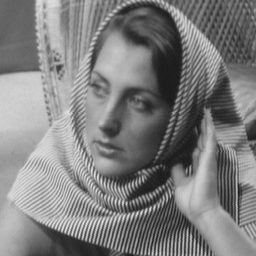
\includegraphics[width=\linewidth]{barbara256.png}
        \caption{Given image}
    \end{subfigure}
    \begin{subfigure}{0.48\linewidth}
        \centering
        \includegraphics[width=\linewidth]{barbara256,σ_noise20.png}
        \caption{Corrupted with Gaussian noise $\mu=0, \sigma=20$}
    \end{subfigure}
    \caption{Barbara image}
    \label{fig:bo}
\end{figure}
\begin{figure}
    \centering
    \begin{subfigure}{0.48\linewidth}
        \centering
        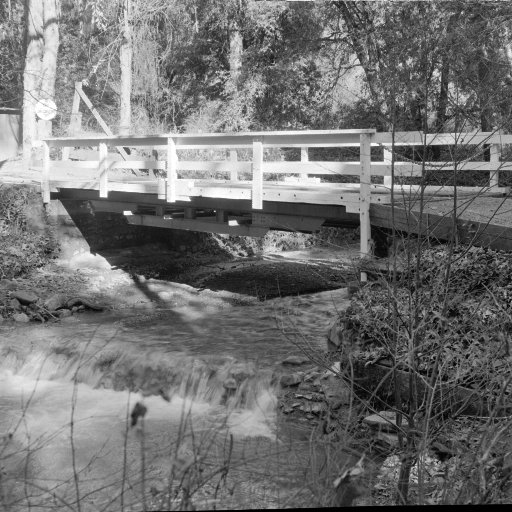
\includegraphics[width=\linewidth]{stream.png}
        \caption{Given image}
    \end{subfigure}
    \begin{subfigure}{0.48\linewidth}
        \centering
        \includegraphics[width=\linewidth]{stream,σ_noise20.png}
        \caption{Corrupted with Gaussian noise $\mu=0, \sigma=20$}
    \end{subfigure}
    \caption{Stream image}
    \label{fig:ko}
\end{figure}
\section{A}
\begin{figure}
    \centering
    \begin{subfigure}{0.48\linewidth}
        \centering
        \includegraphics[width=\linewidth]{barbara256pca2,σ_noise20.png}
        \caption{Barbara}
    \end{subfigure}
    \begin{subfigure}{0.48\linewidth}
        \centering
        \includegraphics[width=\linewidth]{streampca2,σ_noise20.png}
        \caption{Stream}
    \end{subfigure}
    \caption{PCA 1 denoising}
    \label{fig:pca1}
\end{figure}
\section{B}
\ref{fig:pca2} performs better than \ref{fig:pca1}
RMSE values 0.0095 and  0.0109 respectively.
\begin{figure}
    \centering
    \begin{subfigure}{0.48\linewidth}
        \centering
        \includegraphics[width=\linewidth]{barbara256pca2,σ_noise20.png}
        \caption{Barbara}
    \end{subfigure}
    \begin{subfigure}{0.48\linewidth}
        \centering
        \includegraphics[width=\linewidth]{streampca2,σ_noise20.png}
        \caption{Stream}
    \end{subfigure}
    \caption{PCA 2 denoising}
    \label{fig:pca2}
\end{figure}
\section{C}
Bilateral filter maintains the edges but the underlying areas get weird segments/staircasing. With PCA we avoid staircasing as can be seen by comparing both figures. PCA is better.

RMSE numbers are 0.0153 and 0.0170 for barbara and 0.0133, 0.0186 for stream.

Even RMSE numbers of PCA2 are lesser.
\subsection{Bilateral filter on original images}{\label{sec:bfo}}
\ref{fig:bs}, \ref{fig:ks} show the results of bilateral filter applied on the original Barbara and Stream image.

As we go from left to right (increasing $\sigma_s, \sigma_r$), for both images, the image looks smoother but the textures get lost as is evident by focusing on the net in the background of the Barbara image, the text on the house in the Stream image and the multi-layered window in the Stream image. Also, some weird artifacts on the edges became more prominent like at the edges of facial features of Barbara.
\begin{figure}
    \centering
    \begin{subfigure}{0.48\linewidth}
        \centering
        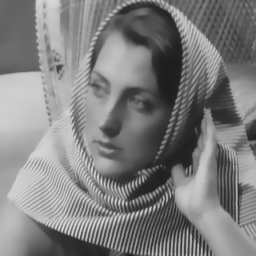
\includegraphics[width=\linewidth]{barbara256,σ_spatial3,σ_range15.png}
        \caption{$\sigma_s=3, \sigma_r=15$}
    \end{subfigure}
    \begin{subfigure}{0.48\linewidth}
        \centering
        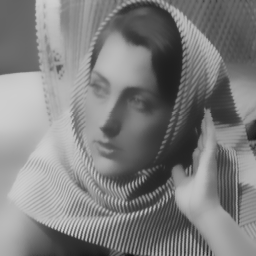
\includegraphics[width=\linewidth]{barbara256,σ_spatial6,σ_range30.png}
        \caption{$\sigma_s=6, \sigma_r=30$}
    \end{subfigure}
    \caption{Bilateral filter on original Barbara image}
    \label{fig:bs}
\end{figure}
\begin{figure}
    \centering
    \begin{subfigure}{0.48\linewidth}
        \centering
        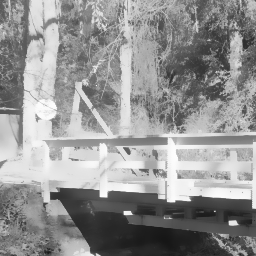
\includegraphics[width=\linewidth]{stream,σ_spatial3,σ_range15.png}
        \caption{$\sigma_s=3, \sigma_r=15$}
    \end{subfigure}
    \begin{subfigure}{0.48\linewidth}
        \centering
        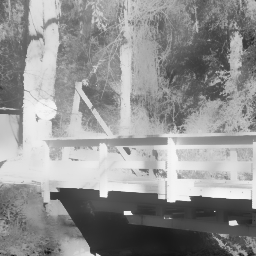
\includegraphics[width=\linewidth]{stream,σ_spatial6,σ_range30.png}
        \caption{$\sigma_s=6, \sigma_r=30$}
    \end{subfigure}
    \caption{Bilateral filter on original Stream image}
    \label{fig:ks}
\end{figure}
\subsection{Bilateral filter on noisy images}
\ref{fig:bn}, \ref{fig:kn} show the results of bilateral filter applied on the noisy Barbara and Stream image.

Bilateral filter of the biggest size $(\sigma_s=3, \sigma_r=15)$ does a good job in noise removal from both the images corrupted by both kind of Gaussian noise. 

We get similar results as in \ref{sec:bfo}, from left to right (increasing $\sigma_s, \sigma_r$), for both images, smoothening increases, the textures get lost and some weird edge artifacts arise. The examples mentioned in \ref{sec:bfo} applies here too.
\begin{figure}
    \centering
    \begin{subfigure}{0.48\linewidth}
        \centering
        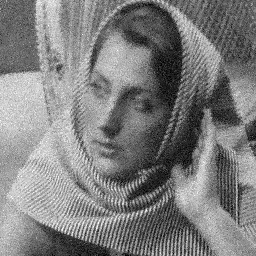
\includegraphics[width=\linewidth]{barbara256,σ_noise20,σ_spatial3,σ_range15.png}
        \caption{$\mu, \sigma = 0, 20, \sigma_s=3, \sigma_r=15$}
    \end{subfigure}
    \begin{subfigure}{0.48\linewidth}
        \centering
        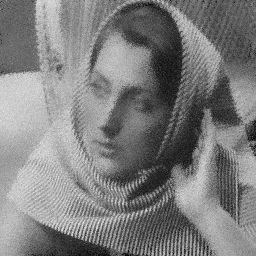
\includegraphics[width=\linewidth]{barbara256,σ_noise20,σ_spatial6,σ_range30.png}
        \caption{$\mu, \sigma = 0, 20, \sigma_s=6, \sigma_r=30$}
    \end{subfigure}
    \caption{Bilateral filter on noisy Barbara image}
    \label{fig:bn}
\end{figure}
\begin{figure}
    \centering
    \begin{subfigure}{0.48\linewidth}
        \centering
        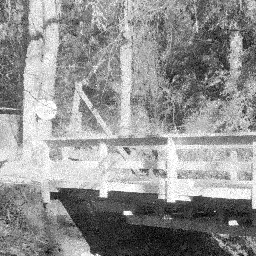
\includegraphics[width=\linewidth]{stream,σ_noise20,σ_spatial3,σ_range15.png}
        \caption{$\mu, \sigma = 0, 20, \sigma_s=3, \sigma_r=15$}
    \end{subfigure}
    \begin{subfigure}{0.48\linewidth}
        \centering
        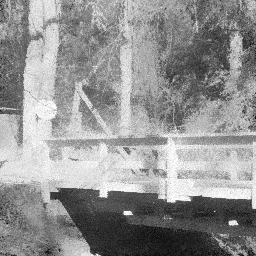
\includegraphics[width=\linewidth]{stream,σ_noise20,σ_spatial6,σ_range30.png}
        \caption{$\mu, \sigma = 0, 20, \sigma_s=6, \sigma_r=30$}
    \end{subfigure}
    \caption{Bilateral filter on noisy Stream image}
    \label{fig:kn}
\end{figure}
{\it Note the size of the filter is such that it includes the points at most ${\lceil3\sigma_s\rceil}$ away from the center point.
}
% \subsection{Bilateral filter creation}
\section{D}
If we clamps the values in the noisy image to [0,255] then the `noise' we get will not follow the Gaussian assumption which PCA requires. But it might not produce drastic differences, only minor differences/artifacting. 
\end{document}